\chapter{Pulsos ultrarrápidos: fundamentos físicos}
\label{ch:Theoretical background}


Este capítulo establece los fundamentos físicos y matemáticos necesarios para comprender la generación y 
evolución de pulsos ultrarrápidos, así como los principios de los algoritmos de aprendizaje automático 
empleados para su optimización. Se parte de la ecuación de propagación no lineal en medios dispersivos y se 
detallan los mecanismos de bloqueo de modos. Posteriormente, se formalizan las técnicas de Machine Learning 
seleccionadas: Algoritmos Genéticos, Redes Neuronales y Optimización Bayesiana.


Debido a la naturaleza ondulatoria de la luz y que esta es una propiedad fundamental de la radiación electromagnética, se exponen los conceptos básicos  

\section{Propagación linear de un pulso}

\section{Técnicas de bloqueo de modos}

El bloqueo de modos (del inglés, mode-locking) constituye la técnica fundamental para la generación de pulsos ópticos en el régimen ultrarrápido. En un oscilador que opera bajo bloqueo de modos en onda continua (CW mode-locking), la duración temporal de los pulsos emitidos es órdenes de magnitud inferior al tiempo de ida y vuelta de la cavidad (round-trip time), el cual dicta de manera estricta la tasa de repetición del sistema. Típicamente, este régimen se caracteriza por la propagación intracavidad de un único pulso ultracorto confinado a una escala de picosegundos o femtosegundos, o bien de un tren de pulsos con espaciamiento temporal constante en el caso de operar bajo bloqueo de modos armónico.

\begin{figure}[h]
    \centering
    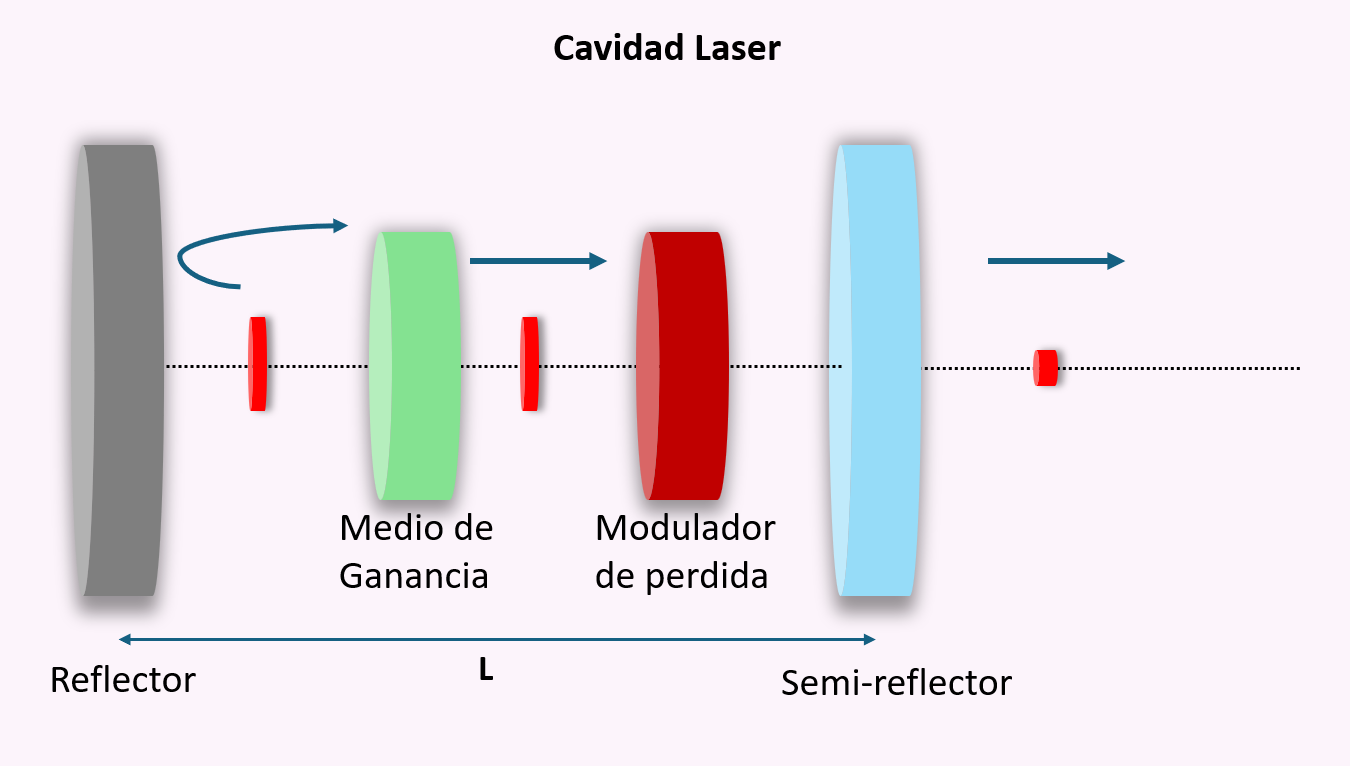
\includegraphics[scale=0.3]{chapters/images/ch3/CavidadLaser_fig3.png}
    \caption{Representación esquemática de la cavidad resonante de un láser de longitud L, diseñada para operar en régimen de bloqueo de modos. El sistema alberga un medio activo (ganancia) y un elemento de modulación (pérdida). La cavidad está delimitada por un espejo de alta reflectancia (HR) en un extremo y un espejo acoplador de salida semitransparente (OC) en el opuesto.}
    \label{fig:CavidadLaser_fig3}
\end{figure}

La arquitectura clásica de un láser de modos bloqueados requiere la integración de un elemento modulador en el interior de la cavidad (véase la Figura \ref{fig:CavidadLaser_fig3}). La propagación del campo electromagnético a través de este componente permite la formación de pulsos sincronizados con los instantes de mínima atenuación impuestos por el modulador. La periodicidad intrínseca de esta modulación coincide con el tiempo de vuelo de ida y vuelta de la cavidad, matemáticamente definido como $T_R=2/Lv_g$, donde $L$ representa la longitud óptica de la cavidad y $v_g$ denota la velocidad de grupo del paquete de ondas en el medio.

\subsection{Procesos inmersos en el bloqueo de modos}

Para establecer y sostener el régimen de bloqueo de modos, es imperativo incorporar un mecanismo (moduladores activos o pasivos fuertemente no lineales) que induzca una relación de fase rígidamente coherente entre los múltiples modos longitudinales resonantes de la cavidad. La dinámica espaciotemporal del pulso ultracorto durante su propagación intracavidad está dictada por una interacción altamente compleja de diversos fenómenos físicos macroscópicos:

    \begin{itemize}
        \item Ganancia. Como en todo oscilador, se requiere un medio activo que provea amplificación suficiente para compensar las pérdidas totales. Mientras que en regímenes monomodo la ganancia es sensible exclusivamente a la potencia promedio, en el bloqueo de modos la elevada intensidad pico de los pulsos ultracortos puede inducir una saturación dinámica y rápida del medio activo (efecto particularmente relevante en láseres de colorante o semiconductores). Este agotamiento abrupto de la ganancia forma asimétricamente el perfil del pulso, facilitando su acortamiento temporal.
        \item Perdida lineal. Engloban la atenuación no dependiente de la intensidad resultante de la transmisión intencionada a través del acoplador de salida, así como la absorción y dispersión parásitas en los componentes ópticos. Un diseño que optimice la relación entre ganancias y pérdidas lineales es insoslayable para suprimir inestabilidades del tipo Q-switching y garantizar la estabilidad macroscópica del tren de pulsos.
        \item Modulación activa. Consiste en la introducción de un elemento acustoóptico o electroóptico (modulador de amplitud o fase) impulsado por un sintetizador de radiofrecuencia externo. Para lograr el bloqueo de modos, la frecuencia de este forzamiento externo debe coincidir con la frecuencia del resonador pasivo, induciendo bandas laterales que acoplan en fase los modos longitudinales adyacentes.
        \item Pérdida saturable (Modulación pasiva de amplitud): Ocurre cuando la atenuación intracavidad responde de manera inversamente proporcional a la intensidad fluente. Este mecanismo no lineal favorece la transmisión de las intensidades pico (reduciendo las pérdidas) y atenúa las componentes de baja intensidad o ruido de fondo. Los dispositivos de pérdida saturable (tales como los Espejos Absorbedores Saturables de Semiconductor o SESAMs, y el efecto de lente de Kerr, KLM) se clasifican en "rápidos" o "lentos" en función del tiempo de relajación de sus portadores relativos a la duración del pulso. Los absorbedores rápidos son excepcionalmente efectivos para regímenes de femtosegundos dado que moldean simétricamente la envolvente del pulso mediante una modulación instantánea.
        \item Modulación de autofase (SPM): Derivada del efecto Kerr óptico, la SPM es un fenómeno paramétrico en el cual el índice de refracción del material depende de la intensidad lumínica transitoria. En osciladores ultrarrápidos, su tiempo de respuesta es cuasi-instantáneo, provocando un desplazamiento de fase no lineal proporcional a la envolvente temporal del pulso, lo que invariablemente se traduce en la generación de nuevas componentes frecuenciales y un severo ensanchamiento espectral.
        \item Dispersión de la velocidad de grupo (GVD): La dependencia de la velocidad de fase con la frecuencia (dispersión cromática) provoca que las distintas componentes espectrales del pulso transiten por la cavidad con velocidades diferenciadas. En un medio de dispersión normal, esto induce un ensanchamiento temporal (chirping) sistemático del pulso. Para contrarrestar esta deformación y preservar la coherencia temporal, es imperativo implementar esquemas de compensación intracavidad (e.g., pares de prismas o espejos fuertemente chirpeados).
        \item Dinámica solitónica: Es el corolario del balance determinista entre la Modulación de autofase (SPM) y una dispersión anómala neta en la cavidad. Mientras la SPM genera un chirp de frecuencia positiva en el frente del pulso, la dispersión anómala invierte este efecto. Su mutua cancelación permite la propagación de "solitones ópticos", paquetes de onda robustos que mantienen una estructura temporal invariante a lo largo de miles de tránsitos intracavidad.
        \item Limitaciones del ancho de banda y filtrado pasivo: La emisión transitable en el oscilador está acotada por el ancho de banda intrínseco del medio de ganancia y la reflectividad espectral de la óptica intracavidad. Por el principio de incertidumbre de tiempo-ancho de banda, el límite de duración temporal mínima de un pulso ultracorto está dictaminado por la máxima anchura espectral que los elementos pasivos permitan oscilar coherentemente, constituyendo el límite fundamental de la técnica.
    \end{itemize}


\subsection{Principios básicos del bloqueo de modos}

La dinámica de oscilación en una cavidad láser está intrínsecamente gobernada por las condiciones de frontera, las cuales definen los modos axiales permitidos. El bloqueo de modos (mode-locking) consiste en el establecimiento de una relación de fase fija y coherente entre estos modos longitudinales. Este fenómeno se induce mediante la incorporación de un mecanismo de modulación intracavidad que genera una perturbación periódica en las pérdidas o en la ganancia del resonador, forzando la oscilación simultánea y sincronizada de múltiples modos. La interferencia constructiva resultante de este acoplamiento de fase da lugar a la formación de pulsos ultracortos de alta intensidad, mientras que la interferencia destructiva en las regiones inter-pulsos minimiza la emisión en el dominio temporal.

\begin{figure}[h]
    \centering
    \begin{minipage}{0.47\textwidth}
        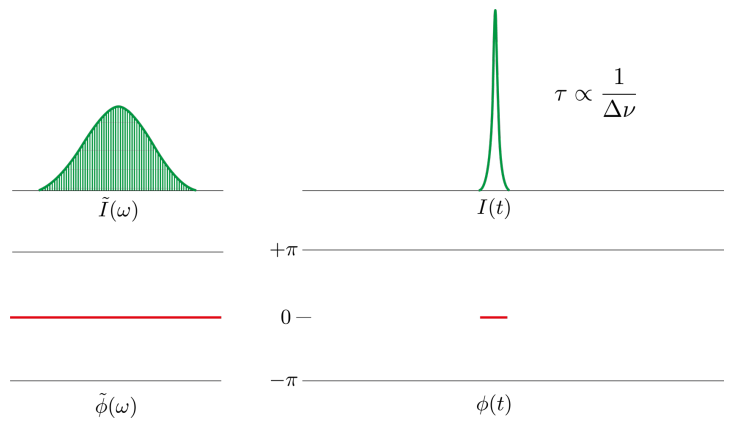
\includegraphics[width=\textwidth]{chapters/images/ch3/Modelocking_fig2a.png}
    \end{minipage}
    \hfill
    \begin{minipage}{0.47\textwidth}
        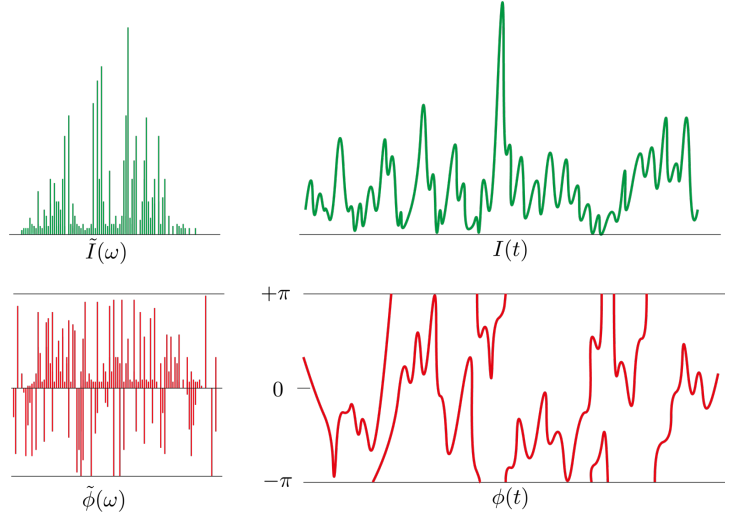
\includegraphics[width=\textwidth]{chapters/images/ch3/Modelocking_fig2b.png}
    \end{minipage}
    \caption{Caracterización del espectro óptico en función de la intensidad $\tilde{I}(\omega)$ y la fase $\tilde{\phi}(\omega)$. a) Régimen de bloqueo de modos (mode-locking): la coherencia de fase entre los múltiples modos longitudinales genera un espectro estructurado y estable, cuya interferencia constructiva resulta en la formación de un pulso ultracorto en el dominio temporal. b) Régimen de emisión multi-modo incoherente: la distribución estocástica de la intensidad y la fase en los modos axiales produce una señal temporal caracterizada por fluctuaciones aleatorias consistentes con ruido óptico, impidiendo la formación de una envolvente de pulso definida .}
    \label{fig:blockMOde&CW}
\end{figure}

La duración del pulso $\tau_p$ es inversamente proporcional al número de modos acoplados, lo que implica que un mayor ancho de banda espectral permite la generación de pulsos temporalmente más estrechos, limitados únicamente por la transformada de Fourier. Para un conjunto de modos axiales con un espaciamiento de frecuencia angular constante $\Delta \omega_{ax}$, una amplitud compleja $\tilde{E}(\omega)$ y una distribución de fase $\phi(\omega)$, el campo eléctrico en el dominio de la frecuencia se expresa como:

\begin{equation}
    \tilde{E}_{tren}(\omega) = \tilde{E}(\omega)e^{i\tilde{\phi}(\omega)} \sum_{m=-\infty}^{\infty} \delta(\omega - m\Delta \omega_{ax})
    \label{eq:6.1}
\end{equation}

donde $m \in \mathbb{Z}$ indexa los modos longitudinales. En el dominio espectral, la intensidad $\tilde{I}_{tren}(\omega) = |\tilde{E}_{tren}(\omega)|^2$ se manifiesta como un peine de frecuencias. Al aplicar la transformada inversa de Fourier a la ecuación \eqref{eq:6.1}, se obtiene la descripción del tren de pulsos en el dominio temporal:

\begin{equation}
    \begin{aligned}
        I_{tren}(t) &= I_p(t) \ast \sum_{m=-\infty}^{\infty}\delta(t - mT_{R})\\
        &= \int_{-\infty}^{\infty} \sum_{m=-\infty}^{\infty}\delta(\tau - mT_{R}) I_p(t - \tau) d\tau\\
        &= \sum_{m=-\infty}^{\infty} \int_{-\infty}^{\infty} \delta(\tau - mT_{R}) I_p(t - \tau) d\tau\\
        &= \sum_{m=-\infty}^{\infty} I_p(t - mT_{R}) 
        \end{aligned}
    \label{eq:6.2}
\end{equation}

donde se ha empleado el hecho de que la transformada de Fourier de un peine de deltas produce otro peine de deltas, y que el producto de dos funciones en el dominio espectral equivale a la convolución de sus transformadas de Fourier inversas. Esta resultado ilustra como el tren de pulsos en el dominio temporal es una suma de pulsos individuales $I_p(t)$, cada uno desplazado temporalmente por un múltiplo entero del período de repetición $T_R$. La duración de cada pulso individual $I_p(t)$ viene dada por $\tau_p$, el cual está determinado por el ancho espectral óptico $\tilde{I}(\nu)$, y una tasa de repetición definida como:

\begin{equation*}
    f_{rep} = \Delta\nu_{ax} = \frac{\Delta\omega_{ax}}{2\pi} = \frac{1}{T_R}.
    \label{eq:tasa_repeticion}
\end{equation*}

Es imperativo distinguir entre la naturaleza espectral de un pulso aislado y la de un tren de pulsos. Mientras que un pulso único presenta un espectro continuo, la periodicidad intrínseca del tren de pulsos impuesta por la cavidad resulta en un espectro discreto o "peine de frecuencias". Como se ilustra en la Figura \ref{fig:blockMOde&CW}, el bloqueo de modos transforma una emisión multi-modo incoherente (ruido) en una estructura temporalmente localizada y altamente estable.

\begin{figure}[h]
    \centering
    \begin{minipage}{0.47\textwidth}
        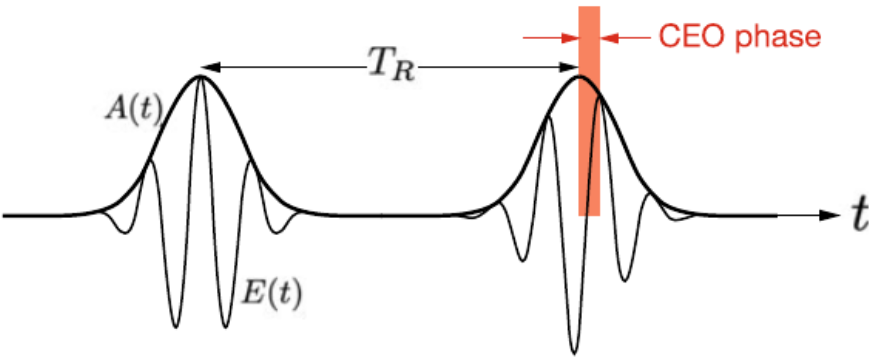
\includegraphics[width=\textwidth]{chapters/images/ch3/CEO_Phase.png}
        \small (a) Dominio temporal.
    \end{minipage}
    \hfill
    \begin{minipage}{0.47\textwidth}
        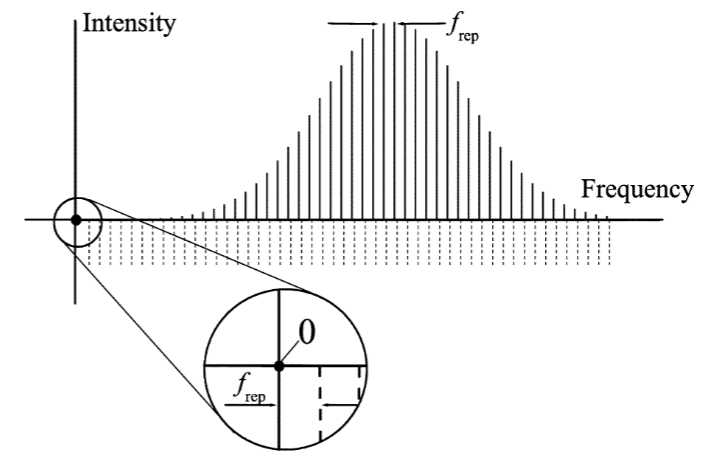
\includegraphics[width=\textwidth]{chapters/images/ch3/equidistantFrecuencyComb.png}
        \small (b) Dominio espectral.
    \end{minipage}
    \caption{
    Dinámica temporal y espectral de un tren de pulsos ultracortos. a) Representación en el dominio temporal donde se ilustra la evolución de la fase portador-envolvente (CEO). La disparidad entre las velocidades de grupo y de fase en la cavidad induce un desplazamiento relativo ($\Delta\phi_{ce}$) del campo eléctrico respecto a la envolvente en cada periodo de repetición $T_R$ \cite{Keller_2022}. b) Representación en el dominio espectral evidenciando la estructura de peine de frecuencias ópticas. El sistema posee dos grados de libertad fundamentales: el intervalo entre modos ($f_{rep} = 1/T_R$) y la frecuencia de compensación portador-envolvente ($f_{CEO}$). En condiciones de dispersión nula, donde las velocidades de fase y grupo coinciden, el campo eléctrico se reproduce idénticamente de pulso a pulso, resultando en un espectro cuyas líneas son múltiplos enteros de $f_{rep}$ ($f_{CEO} = 0$) \cite{keller_2003}.}
    \label{fig:equidistantFrecuencyComb}
\end{figure}

Para la generación de pulsos ultrarrápidos, el láser debe oscilar en tantos modos axiles como sea posible, con una relación de fase constante entre ellas. Diferentes técnicas y métodos existen para establecer esta condición dentro del láser. Todas estas técnicas se denominan "técnicas de bloqueo de modos", por que los modos que forman el peine de frecuencias están bloqueados en fase y tienen una distribución de fase bien definida. Se pueden clasificar en dos categorías principales: bloqueo de modos activo y bloqueo de modos pasivo. El bloqueo de modos activo emplea moduladores externos (acusto-ópticos o electro-ópticos) sincronizados con $T_R$. Por otro lado, el bloqueo de modos pasivo utiliza elementos no lineales, tales como absorbedores saturables (SESAM) o el efecto Kerr óptico, los cuales modulan las pérdidas en función de la intensidad instantánea, permitiendo alcanzar regímenes de femtosegundos

En sistemas de pocos ciclos, cobra importancia un grado de libertad crítico: el desplazamiento de fase portador-envolvente (carrier-envelope phase, CEP). Debido a la dispersión intracavidad, la velocidad de fase y la velocidad de grupo difieren, provocando que el máximo del campo eléctrico se desplace respecto a la envolvente del pulso en cada tránsito. Este fenómeno se traduce en el dominio espectral como un desplazamiento global del peine de frecuencias por una cantidad denominada frecuencia de compensación portador-envolvente, $f_{CEO}$. Así, la frecuencia de cada diente del peine queda definida por $f_m = m f_{rep} + f_{CEO}$, parámetro fundamental en metrología de frecuencias y óptica de campo fuerte.




\section{Solitones}









\section{Bloqueo de modos activo}

El bloqueo de modos activo es una de las primeras técnicas desarrolladas para generar pulsos ultrarrápidos. Consiste en la introducción de un modulador intracavidad, el cual puede ser de tipo acusto-óptico o electro-óptico, que modula periódicamente las pérdidas o la ganancia del resonador. Para lograr el bloqueo de modos, la frecuencia de este forzamiento externo debe coincidir con la frecuencia del resonador pasivo, induciendo bandas laterales que acoplan en fase los modos longitudinales adyacentes. La radiación inicial del láser es reducida una y otra vez en su transito por el modulador, hasta que se alcanza un régimen de oscilación estable donde los modos axiales están acoplados en fase, dando lugar a la formación de pulsos ultracortos. 

\subsection{Pulsos solitónicos en régimen de bloqueo de modos}

Bajo el actuar de ambos GDD y SPM, el régimen de bloqueo de modos puede evolucionar hacia la formación de solitones ópticos, los cuales son paquetes de onda que mantienen su forma temporal invariante a lo largo de la propagación en la cavidad. Este fenómeno ocurre cuando el efecto de modulación de autofase (SPM) induce un chirp positivo en el frente del pulso, mientras que la dispersión anómala produce un chirp negativo, resultando en una mutua cancelación que estabiliza la forma del pulso. Un modulador de pérdida sinusoidal como el ofrecido por un modulador acusto-óptico, no tendrá un efecto muy fuerte sobre la formación del solitón debido a que su duración temporal es mucho más larga que la duración del pulso. 

Los operadores correspondientes a los efectos de SPM y GDD en la ecuación maestra de Haus se pueden expresar como:

\begin{equation}
    \Delta A_4 = -i\delta|A|^2 A(T, t),
    \label{eq:SPM_change}
\end{equation}

mientras que para GDD

\begin{equation}
    \Delta A_5 = iD\frac{\partial^2}{\partial t^2} A(T, t).
    \label{eq:GDD_change}
\end{equation}

De la forma base de la ecuación maestra de Haus (ecuación. (\ref{})), se puede obtener la ecuación maestra para el régimen solitónico de bloqueo de modos activo, la cual se expresa como:

\begin{equation}
    T_R\frac{\partial}{\partial t} A(T, t) = \bigg[iD\frac{\partial^2}{\partial t^2}  - i\delta |A|^2  \bigg] A(T, t)
    + \bigg[g - l + D_g \frac{\partial^2}{\partial t^2} - M(1 - cos(\omega_m t)) \bigg] A(T, t) = 0
    \label{eq:Haus_soliton}
\end{equation}

La primera parte de la ecuación (\ref{eq:Haus_soliton}) es la ecuación de Schrödinger no lineal (ecuación. (\ref{})), cuya solución conocemos para GDD $ < 0$ y $n_2 > 0$ (solitón fundamental). Materiales láser con un ancho de banda de ganancia lo suficientemente grande para generar pulsos ultracortos también cumplirán que $D_g = \frac{g}{\Omega_g^2} \ll 1$. Esto junto el hecho ya comentado de la modulación de pérdida sinusoidal no tendrá un efecto muy fuerte sobre la formación del solitón, nos permite ver que la primera parte de la ecuación (\ref{eq:Haus_soliton}) será dominante en la dinámica del pulso, relegando así el carácter del segundo término a un actor perturbativo. La solución de esta ecuación maestra se halla por  medio de la teoría de perturbaciones solitónicas, en donde la solución con forma Gaussiana es reemplazada por una forma de secante hiperbólica. Los términos debidos a ganancia y pérdida por  modulación pasan a tener un papel fundamental en la estabilización del pulso solitónico, ya que el equilibrio entre ambos es el que determina la energía del pulso.

Un pulso de solitón no se forma de forma instantánea en el resonador. Esto sucede luego que un pulso inicial recorre cierta cantidad de veces por la cavidad y tras estabilizarse resulta en un pulso de solitón. Supongamos un pulso inicial Gaussiano con una duración determinada. Tras miles de recorridos en el resonador, el sistema evoluciona hacia un pulso en estado estacionario con características de solitón, que tiene una duración  mucho menor. Dentro de los primeros 100 recorridos en el resonador, el pulso Gaussiano inicial se convierte en un pulso de solitón. La energía del pulso inicial que no logra ajustarse a la forma del solitón se distribuye en el denominado continuo. El continuo es una parte del pulso con menor intensidad que no puede formar parte del solitón debido a las faltas de balance entre los efectos no lineales y dispersivos. Dado que el continuo tiene una menor intensidad, la SPM es insuficiente para contrarrestar el ensanchamiento temporal causado por la dispersión. Como resultado, el continuo se expande temporalmente. Cuando el continuo se ensancha lo suficiente, experimenta mayores perdidas debido al modulador de perdidas, lo que hace que el continuo disminuya con el tiempo (Fig. (\ref{fig:time_evolution_Nd:YAG})).

En el marco de referencia del solitón, este experimenta un desplazamiento periódico de fase debido al efecto Kerr (referenciar SECCIÓN). Este desplazamiento de fase genera interferencias periódicas entre el solitón y el continuo. Dichas interferencias desaparecerán gradualmente a medida que el continuo decae, dejando únicamente al solitón.

\begin{figure}
    \centering
    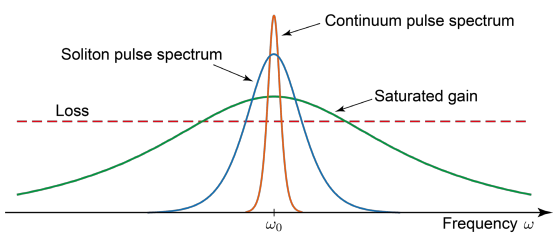
\includegraphics[width=0.8\linewidth]{chapters/images/ch3/saturable_gain.png}
    \caption{La ganancia se satura por el solitón. Sin embargo, ya que el continuo se reduce espectralmente, este verá una mayor ganancia e incremento. La perdida adicional llega únicamente por medio del modulador de perdida, lo cual previene la inestabilidad en el solitón.}
    \label{fig:saturable_gain}
\end{figure}

Para obtener solitones aún más cortos se puede reducir la dispersión del sistema. Sin embargo, una dispersión insuficiente causa que el continuo no se ensanche lo suficientemente rápido para ser absorbido por el modulador de perdidas, lo que lleva a inestabilidades. Después de $10000$ recorridos, estas inestabilidades provocan la formación de los denominados pulsos satélites (pulso más largos y con menor intensidad), que rompen la simetría del pulso propagándose frente al solitón.

Existe un límite en que tanto puede reducirse la duración de los solitones mientras se mantienen estables frente al continuo. Cuando el continuo no decae adecuadamente, el sistema se vuelve inestable y puede generar pulsos adicionales.

El continuo es un pulso residual generado por las perdidas en el modulador, el acoplador de salida y la dispersión del material. Dado que tiene una intensidad mucho menor, no puede mantener el balance entre SPM y la dispersión de grupo negativa (Fig. \ref{fig:saturable_gain})). Este continuo ensanchado eventualmente es suprimido por las mayores perdidas, introduciéndose por el modulador acusto-óptico (Fig. (\ref{fig:GDDbutnoSPMcontinuum})).




